\section{Logical View}
Dette kapitel beskriver systemets opdeling i delsystemer. Her ser vi på de funktionaliteter som systemmet giver til brugeren. 

\subsection{Oversigt}
\logicalview{0.80}{PKG}{System}{System}

For at gøre systemet overskuelig har vi inddelt systemet i flere lag. Således at vi adskiller \Gls{brugergraenseflade} og \Gls{forretningslogik} samt \gls{DAL}. I figur \ref{fig:System_PKG} kan det ses at hver af de store pakker er inddelt i flere små pakker som hver har deres eget ansvar hvilket vil blive beskrevet i følgende afsnit.

\newpage
\subsection{Arkitektursignifikante designpakker	}
\subsubsection{GUI pakken}
Den grafiske brugergrænseflade er først og fremmest lavet ud fra et design som Katrines Kælder
har ønsket. Dette design er baseret på det eksisterende kasseaparats tastatur og mærkater, således
at overgangen fra at skulle bruge det gamle kasseaparat til det nye ville mindskes.
Hertil er der blevet tegnet et skitse som kunne bruges til at lave et mock-up af den kommende GUI. På figur \ref{fig:GUTskitse} kan skitsen af GUI'en ses.\newline

\begin{figure}[H]
\centering
	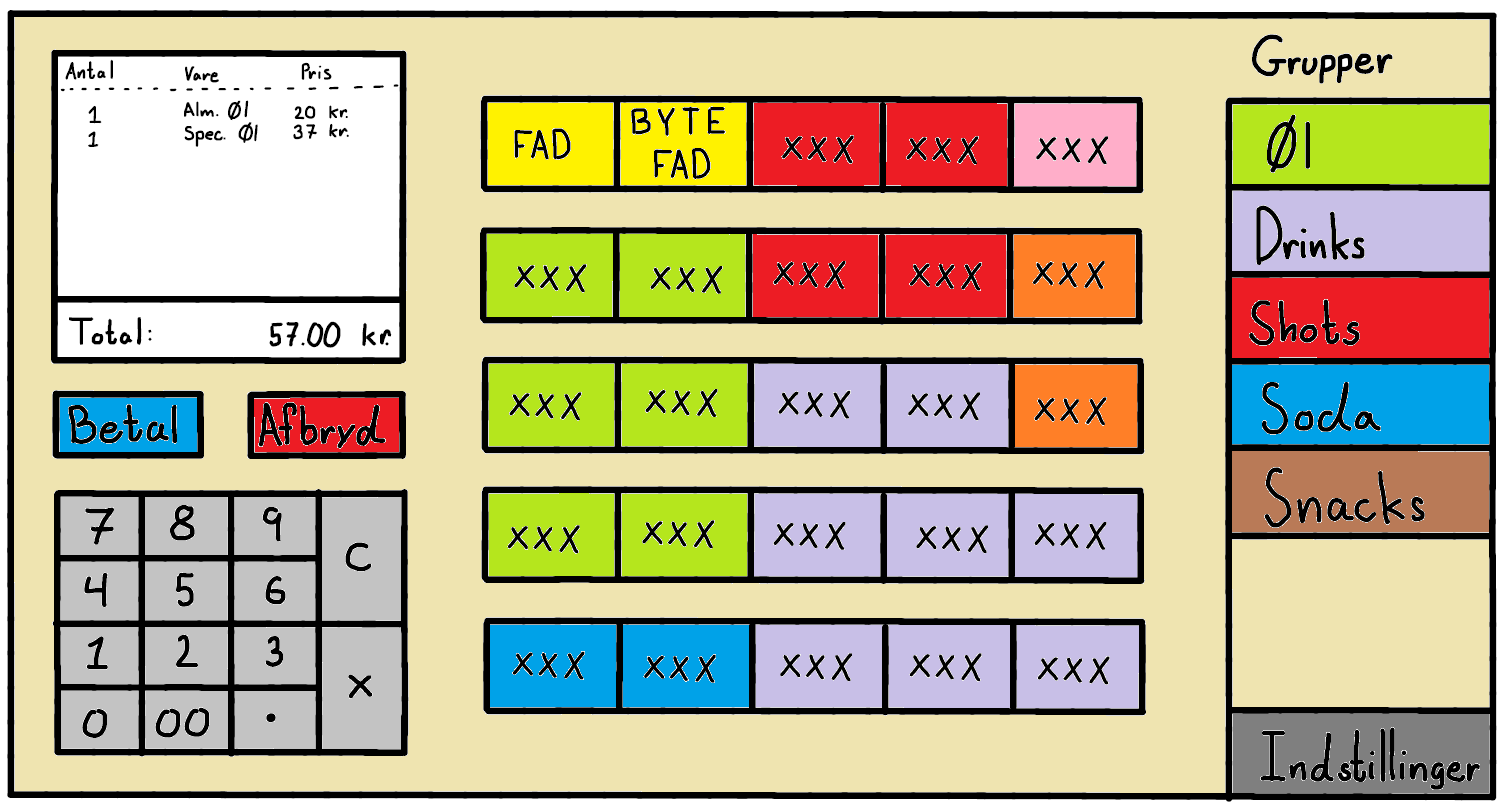
\includegraphics[scale=0.5]{Kravspecifikation/Interface/Interface1F.png}
	\caption{Skitse af GUI}
	\label{fig:GUTskitse}
\end{figure}

\subsubsection{Mock-up}
Det første mock-up blev lavet som en ren illustrativ GUI uden nogen form for funktionalitet. Hertil
blev den lavet uden fornemmelse for hvad der var smart men kun med tankerne om hvordan den
kunne ligne det gamle kasseaparats tastatur. På figur \ref{fig:GUIMock} kan udkastet til GUI'en ses.
\begin{figure}[H]
\centering
	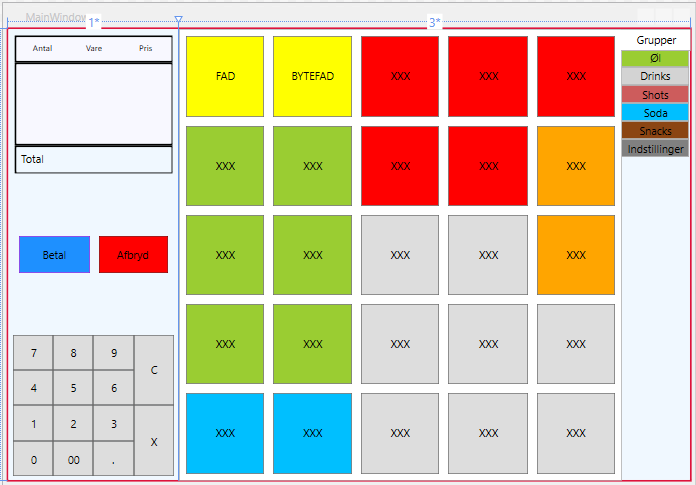
\includegraphics[scale=0.8]{Rapport/GUIMockUp.PNG}
	\caption{Mock up af GUI}
	\label{fig:GUIMock}
\end{figure}
\subsubsection{MVVM}
Da det første mock-up var lavet gik der et sprint hvor der intet GUI blev lavet. Sprintet var mere fokuseret på business logik. Herefter blev der taget fat i GUI’en igen hvor selv hovedvinduet blev delt i tre
UserContents. Dette var smart da det blev aftalt at GUI’en skulle laves efter MVVM princippet
og her kunne de tre usercontents så repræsentere et view hver. Til hver af disse views skulle der så
laves en tilhørende viewModel som kunne hente data fra businesslogikken således at Viewet ikke
skulle tænke på dette selv. Den tilhørende viewmodel skulle nemlig modellere viewet alt efter hvad
der skete i businesslogikken. Dette blev gjort med Bindings fra View til Viewmodel, Og Events fra
businesslogik til Viewmodel.
Selve udseendet af GUI’en blev præget meget af Resources der skulle gøre det hele mere ensartet.
Hertil er der blevet dataTemplates, styles og bindings mm.
Den færdige GUI kom til i sin enkelthed at ligne det mock-up der blev lavet, men der kom meget
mere fokus på hvilke controls der var smarte, og hvilke der ikke var smarte og så fik den en fin
afpusning der gjorde den pænere at se på. På figur \ref{fig:GUIFinal} kan der ses hvor dan GUI'ens endelige udsende blev.

\begin{figure}[H]
\centering
	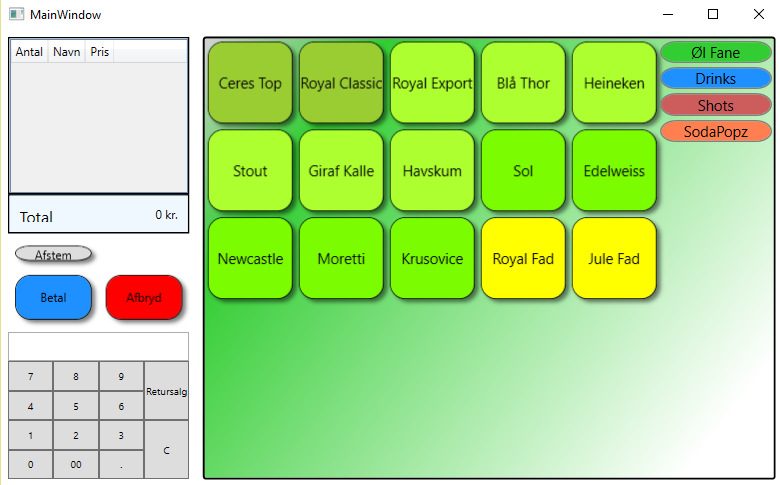
\includegraphics[scale=0.8]{Rapport/GUIFinal.PNG}
	\caption{Endelig udgave af GUI}
	\label{fig:GUIFinal}
\end{figure}

\subsubsection{Dynamik}
Selvom det ikke er til at se i figur \ref{fig:GUIFinal} så er alle produktknapperne dynamisk oprettede. 
En vigtig del af GUI designet var at det skulle være nemt at tilføje/fjerne de produkter der blev solgt.
Dette har vi opnået ved at lade ViewModel stå for at oprette knapperne, dette er gjort ved at have \texttt{ObservableCollections} som der er lavet databind på i \texttt{XAML} koden.
De \texttt{ObservableCollections} gør også at \texttt{XAML} koden kun beskriver hvordan udseendet skal være, da alle knapperne ligger i den \texttt{ObservableCollection}


\newpage
\subsubsection{WebApi pakken}
\textbf{Controllers}
\newline
For at kunne tilgå data fra databasen i vores web interface har vi implementeret et REST api. Til dette har vi brugt en ASP.NETs indbyggede facilitteter \texttt{ApiController} ved at nedarve denne skal vi blot implementere \texttt{Get}, \texttt{Put}, \texttt{Post} og \texttt{Delete} funktionere i vores controllere.

\Diagram{0.85}{CLASS}{WebApi/Controllers}{Web controllers}{LogicalView}

Som det kan ses i figur \ref{fig:WebApi/Controllers_CLASS} er der mange controllere der er faktisk en til alle de typer data vi ønsker at kunne hente ud fra databasen. Desuden bruger alle Controllerne noget kaldt et \texttt{DTO} som står for \texttt{Data transfer object}, disse bliver brugt for at afkoble database fra brugeren af data.
\newline

\textbf{Models}

I figur \ref{fig:WebApi/Controllers_MODEL} ses \texttt{DTO'erne} disse er blot klasser der kun indeholder data.

\Diagram{0.75}{MODEL}{WebApi/Controllers}{Web controllers}{LogicalView}

\newpage
\textbf{WebView}
\newline
Til visualisering af data er der anvendt html/CSS/Javascript, disse data kommer fra vores \texttt{Models} som bliver manipuleret af \texttt{Controller}, som brugeren anvender til at ses, tilføje, slette og ændre data, som illustreret på figur \ref{fig:Diagram_WebView}.
\newline
\newline
Under view i Web Api er der tilføjet 3 view, \texttt{Index}, \texttt{Settings}, og \texttt{Statistic}, dette er 3 html sider, hvor der er anvendt bootstrap til style, form elementer, panels og knapper. Her er der også anvendt knockout data binding attributter, disse binder knockout view models til html elementer, som bliver specificeret i et data-binding udtryk. 
\newline
\newline
De forskellige view-models er defineret i en view model javascript fil, hvor de så bliver gemt som knockout Observable Arrays eller observables, med de værdier der står i databasen. 
\newline
\newline
\begin{figure}[H]
	\centering
	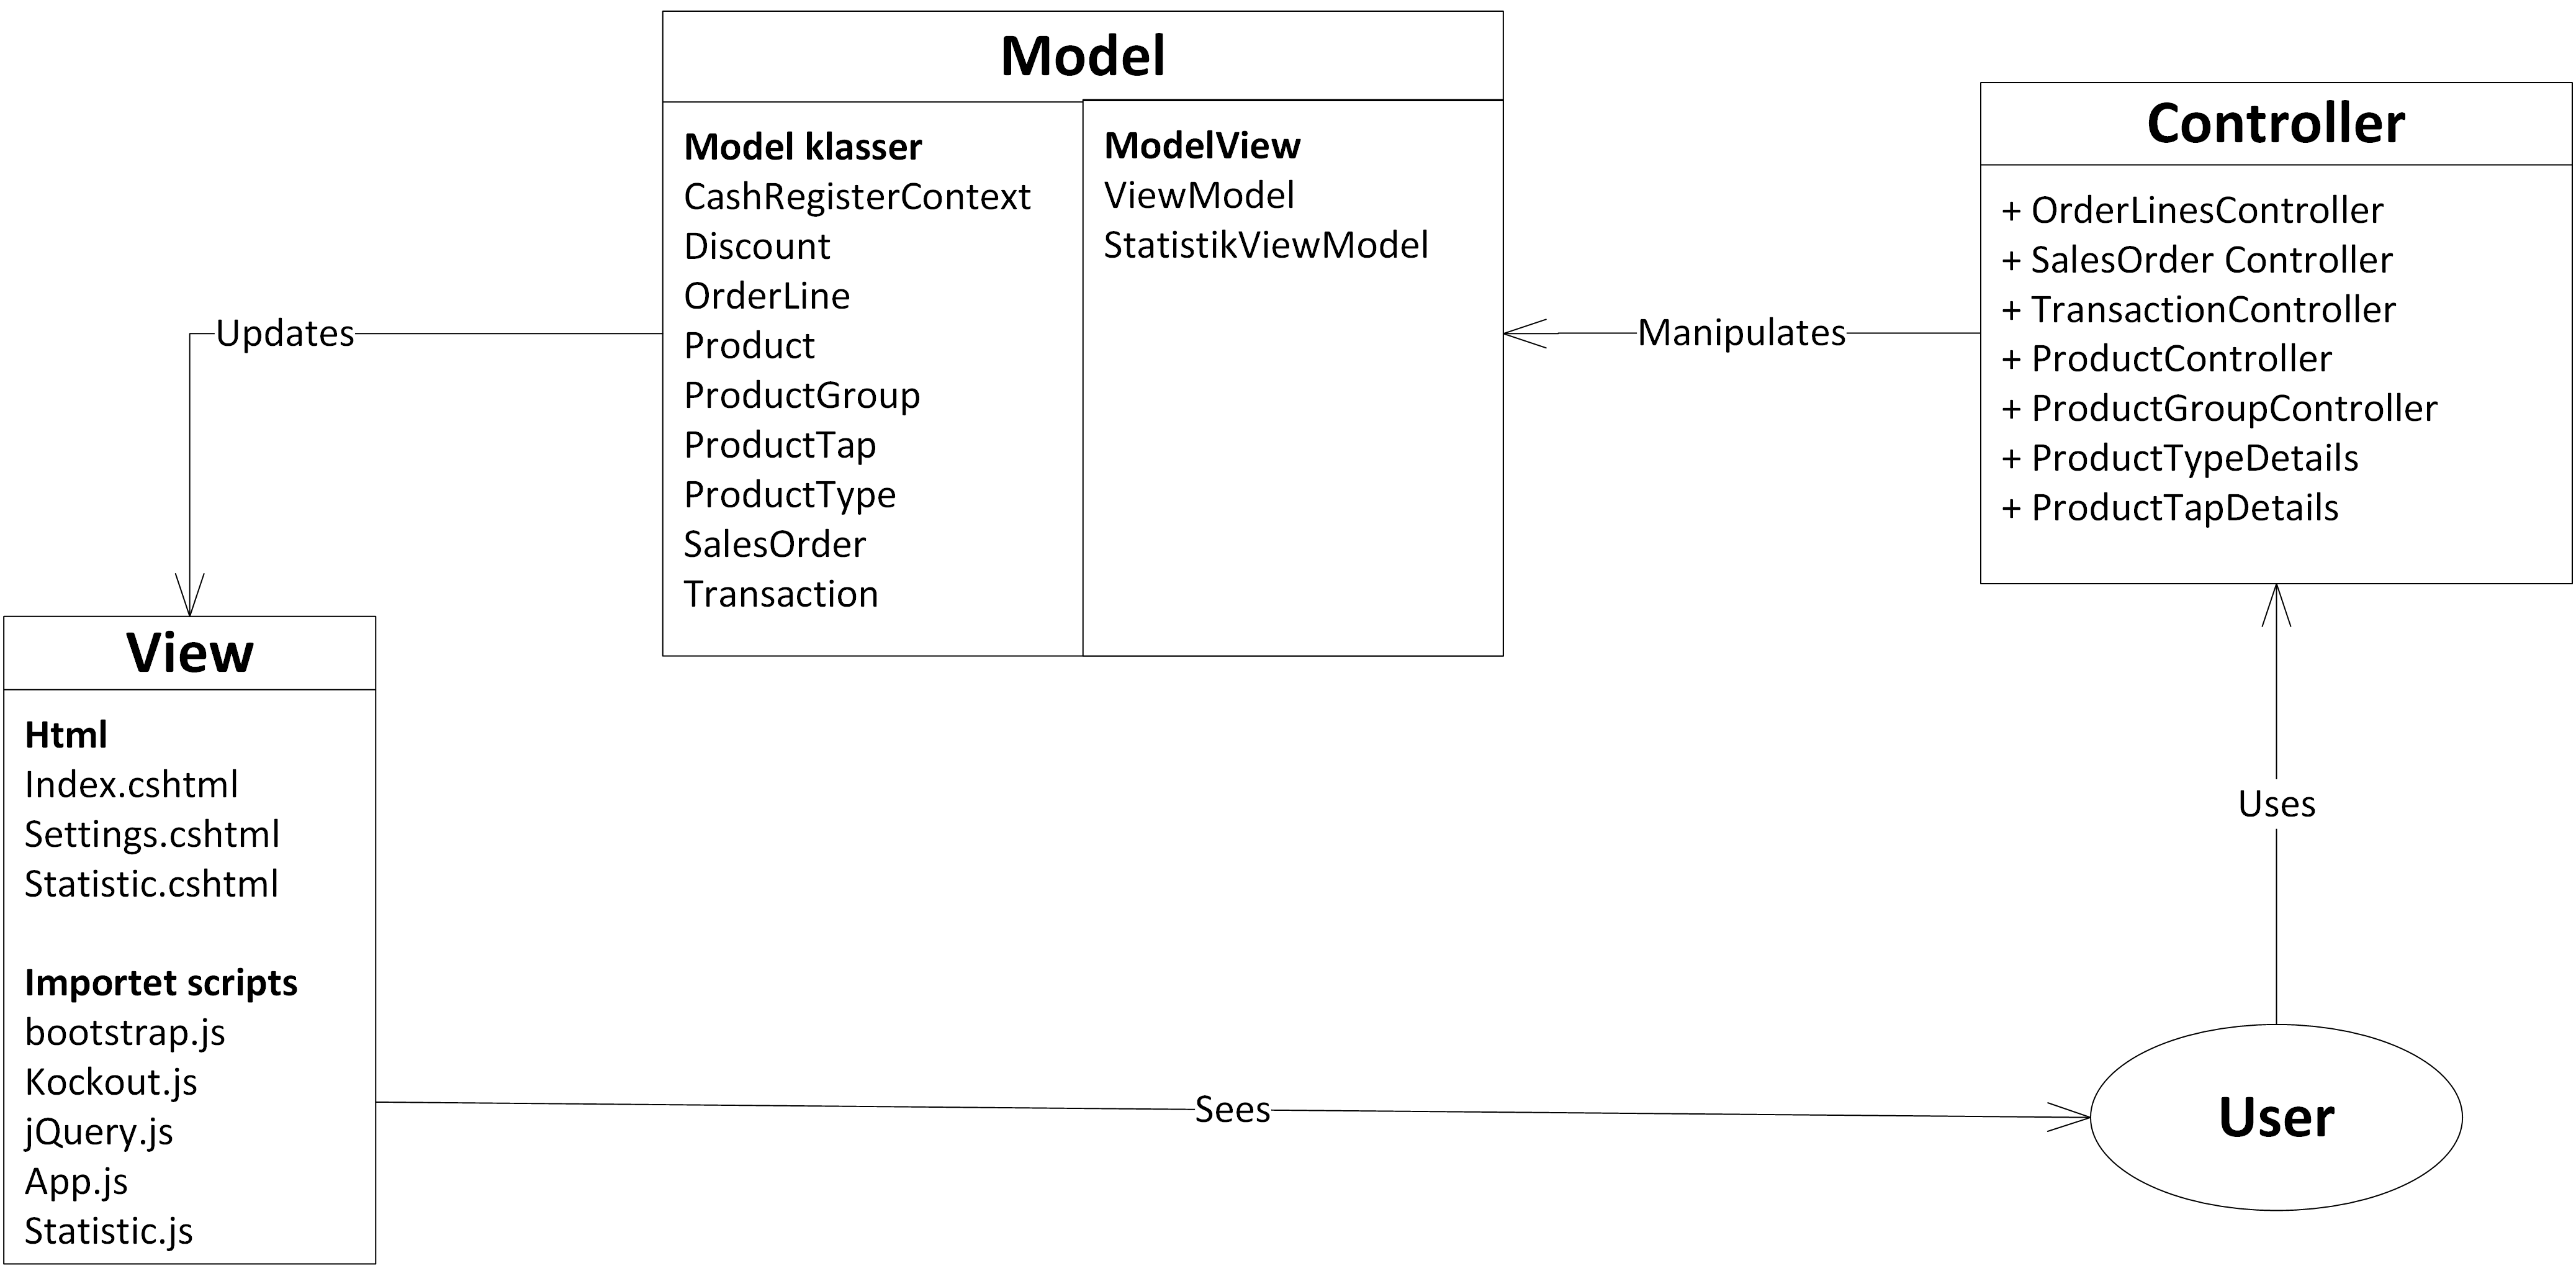
\includegraphics[width=1\textwidth]{N+1/LogicalView/WebApi/WebView/WebViewDiagram.png}
	\caption{Diagram ad WebView}
	\label{fig:Diagram_WebView}
\end{figure}

På figur \ref{fig:WebApi/WebView_SEQ} ses et sequens diagram af WebViewet. Her laver Clienten en http requst til webAPI controlleren, controlleren henter data models der har sit data fra databasen. Det data controlleren har fra models bliver sendt videre til view der formaterer et output via noget html, css og javascript kode. 
\newline
\newline
Ved ændringer af data, som f.eks. kunne være at der bliver tilføjet et objekt, så bliver der udført et asynkron http (Ajax) request, som anvender controllerens POST, til at oprette et nyt object og sætte det i databasen.  

\Diagram{0.85}{SEQ}{WebApi/WebView}{WebView}{LogicalView}

\newpage
\subsubsection{Business Layer pakken}
I dette afsnit beskrives koden i projektets business layer
\subsection{Sales}
%\section{Logical View}
Dette kapitel beskriver systemets opdeling i delsystemer. Her ser vi på de funktionaliteter som systemmet giver til brugeren. 

\subsection{Oversigt}

\subsection{Arkitektursignifikante designpakker	}
\subsubsection{Pakke 1: GUI}


\subsubsection{Pakke 2: Business Layer}
%I dette afsnit beskrives koden i projektets business layer
\subsection{Sales}
%\input{Systemarkitektur/LogicalView/BusinessLayer/Sales}

\subsection{Orders}
%\input{Systemarkitektur/LogicalView/BusinessLayer/Order}

\subsection{Payment}
%\input{Systemarkitektur/LogicalView/BusinessLayer/Payment}

\subsection{Products}
%\input{Systemarkitektur/LogicalView/BusinessLayer/Product}

\subsection{CashDrawers}
%\input{Systemarkitektur/LogicalView/BusinessLayer/CashDrawers}

\subsection{Receipts}
%\input{Systemarkitektur/LogicalView/BusinessLayer/Receipts}

\subsection{Printer}
%\input{Systemarkitektur/LogicalView/BusinessLayer/Printer}

\subsection{Models}
%\input{Systemarkitektur/LogicalView/BusinessLayer/Models}

\subsection{Log}
%\input{Systemarkitektur/LogicalView/BusinessLayer/Log}

\subsection{Database}
%\input{Systemarkitektur/LogicalView/BusinessLayer/Database}

\subsection{Dal}
%\input{Systemarkitektur/LogicalView/BusinessLayer/Dal}




\subsubsection{Pakke 3: Data}

\subsection{Use Case realiseringer	}
\subsubsection{ Use Case 1. realisering	}
\subsubsection{ Use Case 2. realisering	}



\subsection{Orders}
%\input{Systemarkitektur/LogicalView/BusinessLayer/Order}

\subsection{Payment}
%\section{Logical View}
Dette kapitel beskriver systemets opdeling i delsystemer. Her ser vi på de funktionaliteter som systemmet giver til brugeren. 

\subsection{Oversigt}

\subsection{Arkitektursignifikante designpakker	}
\subsubsection{Pakke 1: GUI}


\subsubsection{Pakke 2: Business Layer}
%I dette afsnit beskrives koden i projektets business layer
\subsection{Sales}
%\input{Systemarkitektur/LogicalView/BusinessLayer/Sales}

\subsection{Orders}
%\input{Systemarkitektur/LogicalView/BusinessLayer/Order}

\subsection{Payment}
%\input{Systemarkitektur/LogicalView/BusinessLayer/Payment}

\subsection{Products}
%\input{Systemarkitektur/LogicalView/BusinessLayer/Product}

\subsection{CashDrawers}
%\input{Systemarkitektur/LogicalView/BusinessLayer/CashDrawers}

\subsection{Receipts}
%\input{Systemarkitektur/LogicalView/BusinessLayer/Receipts}

\subsection{Printer}
%\input{Systemarkitektur/LogicalView/BusinessLayer/Printer}

\subsection{Models}
%\input{Systemarkitektur/LogicalView/BusinessLayer/Models}

\subsection{Log}
%\input{Systemarkitektur/LogicalView/BusinessLayer/Log}

\subsection{Database}
%\input{Systemarkitektur/LogicalView/BusinessLayer/Database}

\subsection{Dal}
%\input{Systemarkitektur/LogicalView/BusinessLayer/Dal}




\subsubsection{Pakke 3: Data}

\subsection{Use Case realiseringer	}
\subsubsection{ Use Case 1. realisering	}
\subsubsection{ Use Case 2. realisering	}



\subsection{Products}
%\input{Systemarkitektur/LogicalView/BusinessLayer/Product}

\subsection{CashDrawers}
%\section{Logical View}
Dette kapitel beskriver systemets opdeling i delsystemer. Her ser vi på de funktionaliteter som systemmet giver til brugeren. 

\subsection{Oversigt}

\subsection{Arkitektursignifikante designpakker	}
\subsubsection{Pakke 1: GUI}


\subsubsection{Pakke 2: Business Layer}
%I dette afsnit beskrives koden i projektets business layer
\subsection{Sales}
%\input{Systemarkitektur/LogicalView/BusinessLayer/Sales}

\subsection{Orders}
%\input{Systemarkitektur/LogicalView/BusinessLayer/Order}

\subsection{Payment}
%\input{Systemarkitektur/LogicalView/BusinessLayer/Payment}

\subsection{Products}
%\input{Systemarkitektur/LogicalView/BusinessLayer/Product}

\subsection{CashDrawers}
%\input{Systemarkitektur/LogicalView/BusinessLayer/CashDrawers}

\subsection{Receipts}
%\input{Systemarkitektur/LogicalView/BusinessLayer/Receipts}

\subsection{Printer}
%\input{Systemarkitektur/LogicalView/BusinessLayer/Printer}

\subsection{Models}
%\input{Systemarkitektur/LogicalView/BusinessLayer/Models}

\subsection{Log}
%\input{Systemarkitektur/LogicalView/BusinessLayer/Log}

\subsection{Database}
%\input{Systemarkitektur/LogicalView/BusinessLayer/Database}

\subsection{Dal}
%\input{Systemarkitektur/LogicalView/BusinessLayer/Dal}




\subsubsection{Pakke 3: Data}

\subsection{Use Case realiseringer	}
\subsubsection{ Use Case 1. realisering	}
\subsubsection{ Use Case 2. realisering	}



\subsection{Receipts}
%\section{Logical View}
Dette kapitel beskriver systemets opdeling i delsystemer. Her ser vi på de funktionaliteter som systemmet giver til brugeren. 

\subsection{Oversigt}

\subsection{Arkitektursignifikante designpakker	}
\subsubsection{Pakke 1: GUI}


\subsubsection{Pakke 2: Business Layer}
%I dette afsnit beskrives koden i projektets business layer
\subsection{Sales}
%\input{Systemarkitektur/LogicalView/BusinessLayer/Sales}

\subsection{Orders}
%\input{Systemarkitektur/LogicalView/BusinessLayer/Order}

\subsection{Payment}
%\input{Systemarkitektur/LogicalView/BusinessLayer/Payment}

\subsection{Products}
%\input{Systemarkitektur/LogicalView/BusinessLayer/Product}

\subsection{CashDrawers}
%\input{Systemarkitektur/LogicalView/BusinessLayer/CashDrawers}

\subsection{Receipts}
%\input{Systemarkitektur/LogicalView/BusinessLayer/Receipts}

\subsection{Printer}
%\input{Systemarkitektur/LogicalView/BusinessLayer/Printer}

\subsection{Models}
%\input{Systemarkitektur/LogicalView/BusinessLayer/Models}

\subsection{Log}
%\input{Systemarkitektur/LogicalView/BusinessLayer/Log}

\subsection{Database}
%\input{Systemarkitektur/LogicalView/BusinessLayer/Database}

\subsection{Dal}
%\input{Systemarkitektur/LogicalView/BusinessLayer/Dal}




\subsubsection{Pakke 3: Data}

\subsection{Use Case realiseringer	}
\subsubsection{ Use Case 1. realisering	}
\subsubsection{ Use Case 2. realisering	}



\subsection{Printer}
%\textbf{Printer pakken}
\newline
Printer pakken er lavet for at gøre det muligt for programmet at udskrive kvitteringer samt at udskrive afstemningen af kassen.
Til dette er der lavet et interface \texttt{IPrinter}. \texttt{IPrinter} er lavet for at gøre det nemt at udskifte printer implementationen.
Interfacet er lavet til at modtage en linje ad gangen.
Selve klassen \texttt{ReceiptPrinter} er lavet til at kunne printe via Windows Printer Dialogen til standard printeren.

\logicalview{0.55}{CLASS}{Printer}{pakken Printer}


\subsection{Models}
%\section{Logical View}
Dette kapitel beskriver systemets opdeling i delsystemer. Her ser vi på de funktionaliteter som systemmet giver til brugeren. 

\subsection{Oversigt}

\subsection{Arkitektursignifikante designpakker	}
\subsubsection{Pakke 1: GUI}


\subsubsection{Pakke 2: Business Layer}
%I dette afsnit beskrives koden i projektets business layer
\subsection{Sales}
%\input{Systemarkitektur/LogicalView/BusinessLayer/Sales}

\subsection{Orders}
%\input{Systemarkitektur/LogicalView/BusinessLayer/Order}

\subsection{Payment}
%\input{Systemarkitektur/LogicalView/BusinessLayer/Payment}

\subsection{Products}
%\input{Systemarkitektur/LogicalView/BusinessLayer/Product}

\subsection{CashDrawers}
%\input{Systemarkitektur/LogicalView/BusinessLayer/CashDrawers}

\subsection{Receipts}
%\input{Systemarkitektur/LogicalView/BusinessLayer/Receipts}

\subsection{Printer}
%\input{Systemarkitektur/LogicalView/BusinessLayer/Printer}

\subsection{Models}
%\input{Systemarkitektur/LogicalView/BusinessLayer/Models}

\subsection{Log}
%\input{Systemarkitektur/LogicalView/BusinessLayer/Log}

\subsection{Database}
%\input{Systemarkitektur/LogicalView/BusinessLayer/Database}

\subsection{Dal}
%\input{Systemarkitektur/LogicalView/BusinessLayer/Dal}




\subsubsection{Pakke 3: Data}

\subsection{Use Case realiseringer	}
\subsubsection{ Use Case 1. realisering	}
\subsubsection{ Use Case 2. realisering	}



\subsection{Log}
%\section{Logical View}
Dette kapitel beskriver systemets opdeling i delsystemer. Her ser vi på de funktionaliteter som systemmet giver til brugeren. 

\subsection{Oversigt}

\subsection{Arkitektursignifikante designpakker	}
\subsubsection{Pakke 1: GUI}


\subsubsection{Pakke 2: Business Layer}
%I dette afsnit beskrives koden i projektets business layer
\subsection{Sales}
%\input{Systemarkitektur/LogicalView/BusinessLayer/Sales}

\subsection{Orders}
%\input{Systemarkitektur/LogicalView/BusinessLayer/Order}

\subsection{Payment}
%\input{Systemarkitektur/LogicalView/BusinessLayer/Payment}

\subsection{Products}
%\input{Systemarkitektur/LogicalView/BusinessLayer/Product}

\subsection{CashDrawers}
%\input{Systemarkitektur/LogicalView/BusinessLayer/CashDrawers}

\subsection{Receipts}
%\input{Systemarkitektur/LogicalView/BusinessLayer/Receipts}

\subsection{Printer}
%\input{Systemarkitektur/LogicalView/BusinessLayer/Printer}

\subsection{Models}
%\input{Systemarkitektur/LogicalView/BusinessLayer/Models}

\subsection{Log}
%\input{Systemarkitektur/LogicalView/BusinessLayer/Log}

\subsection{Database}
%\input{Systemarkitektur/LogicalView/BusinessLayer/Database}

\subsection{Dal}
%\input{Systemarkitektur/LogicalView/BusinessLayer/Dal}




\subsubsection{Pakke 3: Data}

\subsection{Use Case realiseringer	}
\subsubsection{ Use Case 1. realisering	}
\subsubsection{ Use Case 2. realisering	}



\subsection{Database}
%\section{Logical View}
Dette kapitel beskriver systemets opdeling i delsystemer. Her ser vi på de funktionaliteter som systemmet giver til brugeren. 

\subsection{Oversigt}

\subsection{Arkitektursignifikante designpakker	}
\subsubsection{Pakke 1: GUI}


\subsubsection{Pakke 2: Business Layer}
%I dette afsnit beskrives koden i projektets business layer
\subsection{Sales}
%\input{Systemarkitektur/LogicalView/BusinessLayer/Sales}

\subsection{Orders}
%\input{Systemarkitektur/LogicalView/BusinessLayer/Order}

\subsection{Payment}
%\input{Systemarkitektur/LogicalView/BusinessLayer/Payment}

\subsection{Products}
%\input{Systemarkitektur/LogicalView/BusinessLayer/Product}

\subsection{CashDrawers}
%\input{Systemarkitektur/LogicalView/BusinessLayer/CashDrawers}

\subsection{Receipts}
%\input{Systemarkitektur/LogicalView/BusinessLayer/Receipts}

\subsection{Printer}
%\input{Systemarkitektur/LogicalView/BusinessLayer/Printer}

\subsection{Models}
%\input{Systemarkitektur/LogicalView/BusinessLayer/Models}

\subsection{Log}
%\input{Systemarkitektur/LogicalView/BusinessLayer/Log}

\subsection{Database}
%\input{Systemarkitektur/LogicalView/BusinessLayer/Database}

\subsection{Dal}
%\input{Systemarkitektur/LogicalView/BusinessLayer/Dal}




\subsubsection{Pakke 3: Data}

\subsection{Use Case realiseringer	}
\subsubsection{ Use Case 1. realisering	}
\subsubsection{ Use Case 2. realisering	}



\subsection{Dal}
%\section{Logical View}
Dette kapitel beskriver systemets opdeling i delsystemer. Her ser vi på de funktionaliteter som systemmet giver til brugeren. 

\subsection{Oversigt}

\subsection{Arkitektursignifikante designpakker	}
\subsubsection{Pakke 1: GUI}


\subsubsection{Pakke 2: Business Layer}
%I dette afsnit beskrives koden i projektets business layer
\subsection{Sales}
%\input{Systemarkitektur/LogicalView/BusinessLayer/Sales}

\subsection{Orders}
%\input{Systemarkitektur/LogicalView/BusinessLayer/Order}

\subsection{Payment}
%\input{Systemarkitektur/LogicalView/BusinessLayer/Payment}

\subsection{Products}
%\input{Systemarkitektur/LogicalView/BusinessLayer/Product}

\subsection{CashDrawers}
%\input{Systemarkitektur/LogicalView/BusinessLayer/CashDrawers}

\subsection{Receipts}
%\input{Systemarkitektur/LogicalView/BusinessLayer/Receipts}

\subsection{Printer}
%\input{Systemarkitektur/LogicalView/BusinessLayer/Printer}

\subsection{Models}
%\input{Systemarkitektur/LogicalView/BusinessLayer/Models}

\subsection{Log}
%\input{Systemarkitektur/LogicalView/BusinessLayer/Log}

\subsection{Database}
%\input{Systemarkitektur/LogicalView/BusinessLayer/Database}

\subsection{Dal}
%\input{Systemarkitektur/LogicalView/BusinessLayer/Dal}




\subsubsection{Pakke 3: Data}

\subsection{Use Case realiseringer	}
\subsubsection{ Use Case 1. realisering	}
\subsubsection{ Use Case 2. realisering	}





\newpage
\subsubsection{Data pakken}
Database designet er en to delt affære. Der er selve strukturen i databasen også er der koden som tilgår databasen.
Disse beskrive begge i følgende afsnit.

\subsubsection{Database Opbygning}
Opbygning goes here.

\subsubsection{Database kode}
For at kunne tilgå databasen fra C\# blev det besluttet at bruge \gls{EF}. 

\newpage
\subsection{Use Case realiseringer}
\subsubsection{ Use Case 1. realisering	}
%!TEX root = ../../main.tex

\subsection*{Use case 1}
I denne use case ser vi hvor et kontant salg bliver foretaget
\begin{usecase}{1}

\title{ Kontant Salg } 

\field{Mål:}{ At sælge drikkevarer mod kontant betaling }

\field{Initieret af:}{ Bartender }

\field{Aktører:}{ Bartender }

\field{Samtidige forekomster:}{1}

%Preconditions: What must be true on start and worth telling the reader?
\field{Prækondition:}{System skal være tændt og klar}

%Postconditions: What must be true on successful completion and worth telling the reader
\field{Postkondition:}{ Et kontant salg er foretaget }

%Main Success Scenario: A typical, unconditional happy path scenario of success.
\scenario{Hovedscenarie:}{
	\item Bartender vælger drink(s)/pris(er) på systemets touchskærm
	\item Bartender trykker "Total"	
	\item Den samlede pris udregnes
	\item Bartender trykker "Kontant" og skuffen åbnes
	\item Bartender modtager betaling fra kunden
	[Extension 1.1: Kontanter ikke modtaget]
	\item Købet er afsluttet
}


%Extensions: Alternate scenarios of success or failure.
\scenario{Extension 1.1: Kontanter ikke modtaget:}{
		\item Bartender trykker annuller køb
		\item Bartender lukker skuffen
		\item Systemet er klar til næste kunde
}


\end{usecase}



\subsubsection{ Use Case 2. realisering	}
%!TEX root = ../../main.tex

\subsection*{Use case 1}
I denne use case -----
\begin{usecase}

\addtitle{Use Case 2}{ Udskriv Kundebon } 

\addfield{Mål:}{ Systemet får udskrevet en bon med kundens køb på }

\addfield{Initieret af:}{ Bartender }

\addfield{Aktører:}{ Bartender (Primær) }

\addfield{Samtidige forekomster:}{1}

%Preconditions: What must be true on start and worth telling the reader?
\addfield{Prækondition:}{Use Case 1 er gennemført}

%Postconditions: What must be true on successful completion and worth telling the reader
\addfield{Postkondition:}{Kunden (baretender?) modtager bon med køb på }

%Main Success Scenario: A typical, unconditional happy path scenario of success.
\addscenario{Hovedscenarie:}{
	\item Bartender har valgt at der skal udskrives bon (på GUI?)
	\item En dialogbox popper op og bartender bekræfter ønske af bon	
	\item printer udskriver bon  [Ext 1: Der er ikke mere papir]
	\item Bartender udleverer bon til kunde [Ext 2: Kunde er gået]	
}

%Extensions: Alternate scenarios of success or failure.
\addscenario{Udvidelser:}{
	\item[Ex.1] Der er ikke mere papir
		\begin{enumerate}
		\item[1.] Printer stopper. Dialogbox popper op med besked "Fyld papir på printer"
		\item[2.] Bartender fylder papir på printer.
		\item[3.] Der trykkes på 'OK' og fortsættes fra punkt 3
		\end{enumerate}
	\item[Ex.2] Kunde er gået
		\begin{enumerate}
			\item[1.] Bartender smider bon ud
		\end{enumerate}
}


\end{usecase}


\subsubsection{ Use Case 3. realisering	}
%!TEX root = ../../main.tex

\subsection*{Use case 3}
I denne use case, ses der hvordan der udskrives afstemning af kassen
\begin{usecase}{3}

\title{ Kasseafstemning } 

\field{Mål:}{ At Bartenderen har en bon med netto salg og dato udskrevet }

\field{Initieret af:}{ Bartender }

\field{Aktører:}{ Bartender }

\field{Samtidige forekomster:}{1}

%Preconditions: What must be true on start and worth telling the reader?
\field{Prækondition:}{System skal være tændt og klar}

%Postconditions: What must be true on successful completion and worth telling the reader
\field{Postkondition:}{ At netto salget på bonnen stemmer overens med salg indtastet }

%Main Success Scenario: A typical, unconditional happy path scenario of success.
\scenario{Hovedscenarie:}{
	\item Bartender vælger "Indstillinger"
	\item System viser "Indstillinger" menu
	\item Bartender trykker "Afstem"
	\item System viser "Afstem" popup
	[Extension 3.1: Bartender trykker "Annuller"]
	\item Bartender trykker "Godkend"
	\item Printeren printer bonnen
	\item System viser "Hovedmenu"
}


%Extensions: Alternate scenarios of success or failure.
\scenario{Extension 3.1: Bartender trykker Annuller:}{
		\item Systemet går tilbage til Indstillinger menu.
}


\end{usecase}

\subsubsection{ Use Case 9. realisering	}
\textbf{De moduler der realiserer Use Case 9: Tilføj varer til kasseapparat}

\begin{enumerate}
	\item Web API
	\item Database
	\item GUI
\end{enumerate}

Use Case 9 bliver realiseret primært gennem Web API'et som her bruger Database Controllere til at tilgå databasen. I Web API'et kan der indsættes nye produkter og det er samme database som den Business logikken henter i, hvortil der vises på GUI.


\subsubsection{ Use Case 10. realisering	}
\textbf{De Moduler der realiserer Use Case 10: Rediger varer i kasseapparat}

\begin{enumerate}
	\item Web API
	\item Database
	\item GUI
\end{enumerate}

Use Case 10 bliver realiseret primært gennem Wep API'et som her bruger Database Controllere til at tilgå databasen. I Wep API'et kan der redigeres i et allerede eksisterende produkt. Når et produkt er ændret som det ønskes, gemmes det i databasen, of da det er den samme database som business logikken henter fra, kan GUI'en vise det.

\subsubsection{ Use Case 11. realisering	}
\subsection*{Use Case 11}
I denne Use Case ser vi hvordan et produkt bliver fjernet fra databasen.
\begin{usecase}{11}

\title{ Fjern varer fra kasseapparat} 

\field{Mål:}{ At få slettet et produkt fra kasseapparatet }

\field{Initieret af:}{ Admin }

\field{Aktører:}{ Admin (Primær) }

\field{Samtidige forekomster:}{1}

%Preconditions: What must be true on start and worth telling the reader?
\field{Prækondition:}{Der skal være et produkt i databasen}

%Postconditions: What must be true on successful completion and worth telling the reader
\field{Postkondition:}{ Et produkt er slettet og vises ikke på GUI }

%Main Success Scenario: A typical, unconditional happy path scenario of success.
\scenario{Hovedscenarie:}{
	\item Admin vælger link til settings i Wep API
	\item Settings side vises og Admin vælger link til Products 
	\item Products side vises og Admin vælger produkt der skal slettes i produktlisten.
	\item Admin klikker på linket der fjerner produkter \newline
	[Extension 11.1: Admin klikker på andet end link til at fjerne produkt ]
	\item Produktet vises nu ikke i produktlisten
	\item Produktet vises ikke i GUI
}


%Extensions: Alternate scenarios of success or failure.
\scenario{Udvidelser:}{
	\item Extension 11.1: Admin klikker på andet end link til at fjerne produkt
		\begin{enumerate}
		\item[1.] Systemet går ud af produkt side og en anden side vises
		\end{enumerate}		
}


\end{usecase}

\subsubsection{ Use Case 12. realisering	}
\subsection*{Use Case 12}
I denne Use Case ser vi hvordan der vises statistik over solgte produkter i systemet.
\begin{usecase}{12}

\title{ Vis statistik over salg} 

\field{Mål:}{ At få vist statistik over solgte produkter }

\field{Initieret af:}{ Admin }

\field{Aktører:}{ Admin (Primær) }

\field{Samtidige forekomster:}{1}

%Preconditions: What must be true on start and worth telling the reader?
\field{Prækondition:}{Der skal mindt være en igangværende ordre}

%Postconditions: What must be true on successful completion and worth telling the reader
\field{Postkondition:}{ Der vises statistik af solgte produkter og ordrer }

%Main Success Scenario: A typical, unconditional happy path scenario of success.
\scenario{Hovedscenarie:}{
	\item Admin vælger link til Statistik i Wep API
	\item Statistik side vises og Admin vælger ordrer i ordrerlisten
	\item Admin klikker på linket til detaljer om en ordre og detaljer om ordre vises.
	\newline
	[Extension 1.1: Admin klikker på andet end link til at tilføje produkt ]	
}


%Extensions: Alternate scenarios of success or failure.
\scenario{Udvidelser:}{
	\item Extension 1.1: Admin klikker på andet link end link til detaljer
		\begin{enumerate}
		\item[1.] Systemet går ud af produkt side og en anden side vises
		\end{enumerate}		
}


\end{usecase}